\documentclass[twoside]{book}

% Packages required by doxygen
\usepackage{fixltx2e}
\usepackage{calc}
\usepackage{doxygen}
\usepackage{graphicx}
\usepackage[utf8]{inputenc}
\usepackage{makeidx}
\usepackage{multicol}
\usepackage{multirow}
\PassOptionsToPackage{warn}{textcomp}
\usepackage{textcomp}
\usepackage[nointegrals]{wasysym}
\usepackage[table]{xcolor}

% Font selection
\usepackage[T1]{fontenc}
\usepackage{mathptmx}
\usepackage[scaled=.90]{helvet}
\usepackage{courier}
\usepackage{amssymb}
\usepackage{sectsty}
\renewcommand{\familydefault}{\sfdefault}
\allsectionsfont{%
  \fontseries{bc}\selectfont%
  \color{darkgray}%
}
\renewcommand{\DoxyLabelFont}{%
  \fontseries{bc}\selectfont%
  \color{darkgray}%
}
\newcommand{\+}{\discretionary{\mbox{\scriptsize$\hookleftarrow$}}{}{}}

% Page & text layout
\usepackage{geometry}
\geometry{%
  a4paper,%
  top=2.5cm,%
  bottom=2.5cm,%
  left=2.5cm,%
  right=2.5cm%
}
\tolerance=750
\hfuzz=15pt
\hbadness=750
\setlength{\emergencystretch}{15pt}
\setlength{\parindent}{0cm}
\setlength{\parskip}{0.2cm}
\makeatletter
\renewcommand{\paragraph}{%
  \@startsection{paragraph}{4}{0ex}{-1.0ex}{1.0ex}{%
    \normalfont\normalsize\bfseries\SS@parafont%
  }%
}
\renewcommand{\subparagraph}{%
  \@startsection{subparagraph}{5}{0ex}{-1.0ex}{1.0ex}{%
    \normalfont\normalsize\bfseries\SS@subparafont%
  }%
}
\makeatother

% Headers & footers
\usepackage{fancyhdr}
\pagestyle{fancyplain}
\fancyhead[LE]{\fancyplain{}{\bfseries\thepage}}
\fancyhead[CE]{\fancyplain{}{}}
\fancyhead[RE]{\fancyplain{}{\bfseries\leftmark}}
\fancyhead[LO]{\fancyplain{}{\bfseries\rightmark}}
\fancyhead[CO]{\fancyplain{}{}}
\fancyhead[RO]{\fancyplain{}{\bfseries\thepage}}
\fancyfoot[LE]{\fancyplain{}{}}
\fancyfoot[CE]{\fancyplain{}{}}
\fancyfoot[RE]{\fancyplain{}{\bfseries\scriptsize Generated on Fri Dec 19 2014 14\+:17\+:30 for Login\+U\+Idoc by Doxygen }}
\fancyfoot[LO]{\fancyplain{}{\bfseries\scriptsize Generated on Fri Dec 19 2014 14\+:17\+:30 for Login\+U\+Idoc by Doxygen }}
\fancyfoot[CO]{\fancyplain{}{}}
\fancyfoot[RO]{\fancyplain{}{}}
\renewcommand{\footrulewidth}{0.4pt}
\renewcommand{\chaptermark}[1]{%
  \markboth{#1}{}%
}
\renewcommand{\sectionmark}[1]{%
  \markright{\thesection\ #1}%
}

% Indices & bibliography
\usepackage{natbib}
\usepackage[titles]{tocloft}
\setcounter{tocdepth}{3}
\setcounter{secnumdepth}{5}
\makeindex

% Hyperlinks (required, but should be loaded last)
\usepackage{ifpdf}
\ifpdf
  \usepackage[pdftex,pagebackref=true]{hyperref}
\else
  \usepackage[ps2pdf,pagebackref=true]{hyperref}
\fi
\hypersetup{%
  colorlinks=true,%
  linkcolor=blue,%
  citecolor=blue,%
  unicode%
}

% Custom commands
\newcommand{\clearemptydoublepage}{%
  \newpage{\pagestyle{empty}\cleardoublepage}%
}


%===== C O N T E N T S =====

\begin{document}

% Titlepage & ToC
\hypersetup{pageanchor=false,
             bookmarks=true,
             bookmarksnumbered=true,
             pdfencoding=unicode
            }
\pagenumbering{roman}
\begin{titlepage}
\vspace*{7cm}
\begin{center}%
{\Large Login\+U\+Idoc }\\
\vspace*{1cm}
{\large Generated by Doxygen 1.8.8}\\
\vspace*{0.5cm}
{\small Fri Dec 19 2014 14:17:30}\\
\end{center}
\end{titlepage}
\clearemptydoublepage
\tableofcontents
\clearemptydoublepage
\pagenumbering{arabic}
\hypersetup{pageanchor=true}

%--- Begin generated contents ---
\chapter{Hierarchical Index}
\section{Class Hierarchy}
This inheritance list is sorted roughly, but not completely, alphabetically\+:\begin{DoxyCompactList}
\item Action\+Bar\+Activity\begin{DoxyCompactList}
\item \contentsline{section}{com.\+example.\+loginui.\+Main\+Activity}{\pageref{classcom_1_1example_1_1loginui_1_1_main_activity}}{}
\end{DoxyCompactList}
\item Linear\+Layout\begin{DoxyCompactList}
\item \contentsline{section}{com.\+example.\+loginui.\+Field}{\pageref{classcom_1_1example_1_1loginui_1_1_field}}{}
\item \contentsline{section}{com.\+example.\+loginui.\+Password\+Component}{\pageref{classcom_1_1example_1_1loginui_1_1_password_component}}{}
\item \contentsline{section}{com.\+example.\+loginui.\+Registration\+Component}{\pageref{classcom_1_1example_1_1loginui_1_1_registration_component}}{}
\end{DoxyCompactList}
\end{DoxyCompactList}

\chapter{Class Index}
\section{Class List}
Here are the classes, structs, unions and interfaces with brief descriptions\+:\begin{DoxyCompactList}
\item\contentsline{section}{\hyperlink{classcom_1_1example_1_1loginui_1_1_field}{com.\+example.\+loginui.\+Field} }{\pageref{classcom_1_1example_1_1loginui_1_1_field}}{}
\item\contentsline{section}{\hyperlink{classcom_1_1example_1_1loginui_1_1_main_activity}{com.\+example.\+loginui.\+Main\+Activity} }{\pageref{classcom_1_1example_1_1loginui_1_1_main_activity}}{}
\item\contentsline{section}{\hyperlink{classcom_1_1example_1_1loginui_1_1_password_component}{com.\+example.\+loginui.\+Password\+Component} }{\pageref{classcom_1_1example_1_1loginui_1_1_password_component}}{}
\item\contentsline{section}{\hyperlink{classcom_1_1example_1_1loginui_1_1_registration_component}{com.\+example.\+loginui.\+Registration\+Component} }{\pageref{classcom_1_1example_1_1loginui_1_1_registration_component}}{}
\end{DoxyCompactList}

\chapter{Class Documentation}
\hypertarget{classcom_1_1example_1_1loginui_1_1_field}{\section{com.\+example.\+loginui.\+Field Class Reference}
\label{classcom_1_1example_1_1loginui_1_1_field}\index{com.\+example.\+loginui.\+Field@{com.\+example.\+loginui.\+Field}}
}
Inheritance diagram for com.\+example.\+loginui.\+Field\+:\begin{figure}[H]
\begin{center}
\leavevmode
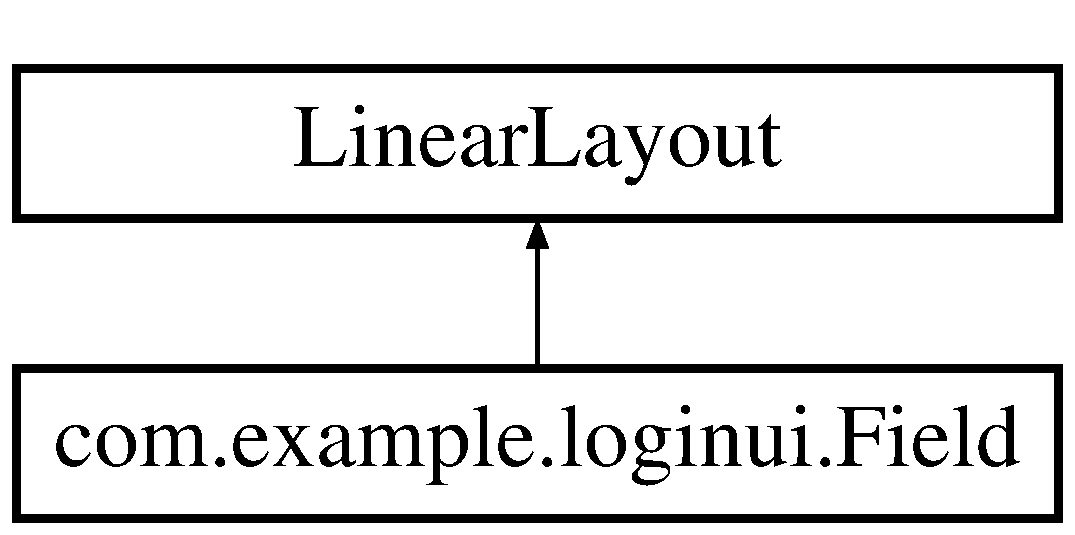
\includegraphics[height=2.000000cm]{classcom_1_1example_1_1loginui_1_1_field}
\end{center}
\end{figure}
\subsection*{Public Member Functions}
\begin{DoxyCompactItemize}
\item 
\hyperlink{classcom_1_1example_1_1loginui_1_1_field_aa5cc967e6f141e0e728a5a448997ae58}{Field} (Context context)
\item 
\hyperlink{classcom_1_1example_1_1loginui_1_1_field_a6e41db5fee5b1751d72af468fc687c7a}{Field} (Context context, String header\+Label)
\item 
\hyperlink{classcom_1_1example_1_1loginui_1_1_field_a02848d9ec2081b327cdb72c132bdf53c}{Field} (Context context, String header\+Label, Boolean required)
\item 
void \hyperlink{classcom_1_1example_1_1loginui_1_1_field_af925595be581e2067e5c0ca7b277f720}{set\+To\+Password\+Field} (boolean bool)
\item 
String \hyperlink{classcom_1_1example_1_1loginui_1_1_field_a50781c5d55fc5761088389c785b99b10}{get\+Text} ()
\item 
void \hyperlink{classcom_1_1example_1_1loginui_1_1_field_a4180d16f564047874c10b272a98c6d0d}{set\+Text\+Color} (int color)
\item 
void \hyperlink{classcom_1_1example_1_1loginui_1_1_field_a6303573051de4a300516af847c883637}{set\+Header\+Color} (int color)
\item 
void \hyperlink{classcom_1_1example_1_1loginui_1_1_field_a7de08a942a8e6240ef010bb56fd674d4}{add\+User} (String s)
\item 
void \hyperlink{classcom_1_1example_1_1loginui_1_1_field_a00e2ba079216104afcf883996db5bed3}{set\+User\+List} (Array\+List$<$ String $>$ list)
\item 
Edit\+Text \hyperlink{classcom_1_1example_1_1loginui_1_1_field_ae1dc2a039ad6fd306c45478d313eaaa5}{get\+Edit\+Text} ()
\item 
String \hyperlink{classcom_1_1example_1_1loginui_1_1_field_acaf75004b06097d8b064f5d30c2a49c6}{get\+Header\+Label} ()
\item 
void \hyperlink{classcom_1_1example_1_1loginui_1_1_field_a539592eabb209f82d58482bff8de5c31}{set\+Header\+Label} (String header\+Label)
\item 
Text\+View \hyperlink{classcom_1_1example_1_1loginui_1_1_field_a3ac22f766a73cb8b782dcfce5ace8002}{get\+Header\+Text\+View} ()
\item 
void \hyperlink{classcom_1_1example_1_1loginui_1_1_field_ae283fc5f4d7351e88503a7bccfa9705f}{set\+Header\+Text\+View} (Text\+View header\+Text\+View)
\item 
Text\+View \hyperlink{classcom_1_1example_1_1loginui_1_1_field_a5719509b2b05db8000637d3bc40f13f2}{get\+Check\+Text\+View} ()
\item 
void \hyperlink{classcom_1_1example_1_1loginui_1_1_field_a7e2c1e43206bc45c4685a2707c1c49b4}{set\+Check\+Text\+View} (Text\+View check\+Text\+View)
\item 
boolean \hyperlink{classcom_1_1example_1_1loginui_1_1_field_a16cda5d55c59d66ecdc2e72e4e873662}{is\+Required} ()
\item 
void \hyperlink{classcom_1_1example_1_1loginui_1_1_field_ae74fd4f0125bdcd4693f228ce0bef35e}{set\+Required} (boolean required)
\item 
boolean \hyperlink{classcom_1_1example_1_1loginui_1_1_field_abd39acfcffe697a5df65f4aef54b3181}{is\+Correct\+Input} ()
\item 
void \hyperlink{classcom_1_1example_1_1loginui_1_1_field_ad78fc604d3d5debc9a8813d13e952f30}{set\+Correct\+Input} (boolean correct\+Input)
\end{DoxyCompactItemize}
\subsection*{Protected Member Functions}
\begin{DoxyCompactItemize}
\item 
boolean \hyperlink{classcom_1_1example_1_1loginui_1_1_field_aa6b2169b6e03936562eb1c72eb951ae8}{is\+Email} (String s)
\end{DoxyCompactItemize}


\subsection{Constructor \& Destructor Documentation}
\hypertarget{classcom_1_1example_1_1loginui_1_1_field_aa5cc967e6f141e0e728a5a448997ae58}{\index{com\+::example\+::loginui\+::\+Field@{com\+::example\+::loginui\+::\+Field}!Field@{Field}}
\index{Field@{Field}!com\+::example\+::loginui\+::\+Field@{com\+::example\+::loginui\+::\+Field}}
\subsubsection[{Field}]{\setlength{\rightskip}{0pt plus 5cm}com.\+example.\+loginui.\+Field.\+Field (
\begin{DoxyParamCaption}
\item[{Context}]{context}
\end{DoxyParamCaption}
)}}\label{classcom_1_1example_1_1loginui_1_1_field_aa5cc967e6f141e0e728a5a448997ae58}
Constructor 
\begin{DoxyParams}{Parameters}
{\em context} & -\/ defines the context \\
\hline
\end{DoxyParams}
\hypertarget{classcom_1_1example_1_1loginui_1_1_field_a6e41db5fee5b1751d72af468fc687c7a}{\index{com\+::example\+::loginui\+::\+Field@{com\+::example\+::loginui\+::\+Field}!Field@{Field}}
\index{Field@{Field}!com\+::example\+::loginui\+::\+Field@{com\+::example\+::loginui\+::\+Field}}
\subsubsection[{Field}]{\setlength{\rightskip}{0pt plus 5cm}com.\+example.\+loginui.\+Field.\+Field (
\begin{DoxyParamCaption}
\item[{Context}]{context, }
\item[{String}]{header\+Label}
\end{DoxyParamCaption}
)}}\label{classcom_1_1example_1_1loginui_1_1_field_a6e41db5fee5b1751d72af468fc687c7a}
Constructor 
\begin{DoxyParams}{Parameters}
{\em context} & -\/ defines context \\
\hline
{\em header\+Label} & -\/ defines the header of the field \\
\hline
\end{DoxyParams}
\hypertarget{classcom_1_1example_1_1loginui_1_1_field_a02848d9ec2081b327cdb72c132bdf53c}{\index{com\+::example\+::loginui\+::\+Field@{com\+::example\+::loginui\+::\+Field}!Field@{Field}}
\index{Field@{Field}!com\+::example\+::loginui\+::\+Field@{com\+::example\+::loginui\+::\+Field}}
\subsubsection[{Field}]{\setlength{\rightskip}{0pt plus 5cm}com.\+example.\+loginui.\+Field.\+Field (
\begin{DoxyParamCaption}
\item[{Context}]{context, }
\item[{String}]{header\+Label, }
\item[{Boolean}]{required}
\end{DoxyParamCaption}
)}}\label{classcom_1_1example_1_1loginui_1_1_field_a02848d9ec2081b327cdb72c132bdf53c}
Constructor 
\begin{DoxyParams}{Parameters}
{\em context} & -\/ defines context \\
\hline
{\em header\+Label} & -\/ defines the header of the field \\
\hline
{\em required} & -\/ define if the field should be required or not \\
\hline
\end{DoxyParams}


\subsection{Member Function Documentation}
\hypertarget{classcom_1_1example_1_1loginui_1_1_field_a7de08a942a8e6240ef010bb56fd674d4}{\index{com\+::example\+::loginui\+::\+Field@{com\+::example\+::loginui\+::\+Field}!add\+User@{add\+User}}
\index{add\+User@{add\+User}!com\+::example\+::loginui\+::\+Field@{com\+::example\+::loginui\+::\+Field}}
\subsubsection[{add\+User}]{\setlength{\rightskip}{0pt plus 5cm}void com.\+example.\+loginui.\+Field.\+add\+User (
\begin{DoxyParamCaption}
\item[{String}]{s}
\end{DoxyParamCaption}
)}}\label{classcom_1_1example_1_1loginui_1_1_field_a7de08a942a8e6240ef010bb56fd674d4}
Add user to the userlist. 
\begin{DoxyParams}{Parameters}
{\em s} & -\/ user name \hyperlink{}{string}. \\
\hline
\end{DoxyParams}
\hypertarget{classcom_1_1example_1_1loginui_1_1_field_a5719509b2b05db8000637d3bc40f13f2}{\index{com\+::example\+::loginui\+::\+Field@{com\+::example\+::loginui\+::\+Field}!get\+Check\+Text\+View@{get\+Check\+Text\+View}}
\index{get\+Check\+Text\+View@{get\+Check\+Text\+View}!com\+::example\+::loginui\+::\+Field@{com\+::example\+::loginui\+::\+Field}}
\subsubsection[{get\+Check\+Text\+View}]{\setlength{\rightskip}{0pt plus 5cm}Text\+View com.\+example.\+loginui.\+Field.\+get\+Check\+Text\+View (
\begin{DoxyParamCaption}
{}
\end{DoxyParamCaption}
)}}\label{classcom_1_1example_1_1loginui_1_1_field_a5719509b2b05db8000637d3bc40f13f2}
Get the check \hyperlink{}{Text\+View} of the \hyperlink{classcom_1_1example_1_1loginui_1_1_field}{Field} \begin{DoxyReturn}{Returns}
\hyperlink{}{Text\+View} 
\end{DoxyReturn}
\hypertarget{classcom_1_1example_1_1loginui_1_1_field_ae1dc2a039ad6fd306c45478d313eaaa5}{\index{com\+::example\+::loginui\+::\+Field@{com\+::example\+::loginui\+::\+Field}!get\+Edit\+Text@{get\+Edit\+Text}}
\index{get\+Edit\+Text@{get\+Edit\+Text}!com\+::example\+::loginui\+::\+Field@{com\+::example\+::loginui\+::\+Field}}
\subsubsection[{get\+Edit\+Text}]{\setlength{\rightskip}{0pt plus 5cm}Edit\+Text com.\+example.\+loginui.\+Field.\+get\+Edit\+Text (
\begin{DoxyParamCaption}
{}
\end{DoxyParamCaption}
)}}\label{classcom_1_1example_1_1loginui_1_1_field_ae1dc2a039ad6fd306c45478d313eaaa5}
Get \hyperlink{}{Edit\+Text} of the \hyperlink{classcom_1_1example_1_1loginui_1_1_field}{Field} \begin{DoxyReturn}{Returns}
\hyperlink{}{Edit\+Text} 
\end{DoxyReturn}
\hypertarget{classcom_1_1example_1_1loginui_1_1_field_acaf75004b06097d8b064f5d30c2a49c6}{\index{com\+::example\+::loginui\+::\+Field@{com\+::example\+::loginui\+::\+Field}!get\+Header\+Label@{get\+Header\+Label}}
\index{get\+Header\+Label@{get\+Header\+Label}!com\+::example\+::loginui\+::\+Field@{com\+::example\+::loginui\+::\+Field}}
\subsubsection[{get\+Header\+Label}]{\setlength{\rightskip}{0pt plus 5cm}String com.\+example.\+loginui.\+Field.\+get\+Header\+Label (
\begin{DoxyParamCaption}
{}
\end{DoxyParamCaption}
)}}\label{classcom_1_1example_1_1loginui_1_1_field_acaf75004b06097d8b064f5d30c2a49c6}
Get the header label of the \hyperlink{classcom_1_1example_1_1loginui_1_1_field}{Field}. \begin{DoxyReturn}{Returns}
\hyperlink{}{String} 
\end{DoxyReturn}
\hypertarget{classcom_1_1example_1_1loginui_1_1_field_a3ac22f766a73cb8b782dcfce5ace8002}{\index{com\+::example\+::loginui\+::\+Field@{com\+::example\+::loginui\+::\+Field}!get\+Header\+Text\+View@{get\+Header\+Text\+View}}
\index{get\+Header\+Text\+View@{get\+Header\+Text\+View}!com\+::example\+::loginui\+::\+Field@{com\+::example\+::loginui\+::\+Field}}
\subsubsection[{get\+Header\+Text\+View}]{\setlength{\rightskip}{0pt plus 5cm}Text\+View com.\+example.\+loginui.\+Field.\+get\+Header\+Text\+View (
\begin{DoxyParamCaption}
{}
\end{DoxyParamCaption}
)}}\label{classcom_1_1example_1_1loginui_1_1_field_a3ac22f766a73cb8b782dcfce5ace8002}
Get the header \hyperlink{}{Text\+View} of the \hyperlink{classcom_1_1example_1_1loginui_1_1_field}{Field} \begin{DoxyReturn}{Returns}
\hyperlink{}{Text\+View} 
\end{DoxyReturn}
\hypertarget{classcom_1_1example_1_1loginui_1_1_field_a50781c5d55fc5761088389c785b99b10}{\index{com\+::example\+::loginui\+::\+Field@{com\+::example\+::loginui\+::\+Field}!get\+Text@{get\+Text}}
\index{get\+Text@{get\+Text}!com\+::example\+::loginui\+::\+Field@{com\+::example\+::loginui\+::\+Field}}
\subsubsection[{get\+Text}]{\setlength{\rightskip}{0pt plus 5cm}String com.\+example.\+loginui.\+Field.\+get\+Text (
\begin{DoxyParamCaption}
{}
\end{DoxyParamCaption}
)}}\label{classcom_1_1example_1_1loginui_1_1_field_a50781c5d55fc5761088389c785b99b10}
Get text from \hyperlink{}{Edit\+Text} in \hyperlink{classcom_1_1example_1_1loginui_1_1_field}{Field} \begin{DoxyReturn}{Returns}
\hyperlink{}{String} 
\end{DoxyReturn}
\hypertarget{classcom_1_1example_1_1loginui_1_1_field_abd39acfcffe697a5df65f4aef54b3181}{\index{com\+::example\+::loginui\+::\+Field@{com\+::example\+::loginui\+::\+Field}!is\+Correct\+Input@{is\+Correct\+Input}}
\index{is\+Correct\+Input@{is\+Correct\+Input}!com\+::example\+::loginui\+::\+Field@{com\+::example\+::loginui\+::\+Field}}
\subsubsection[{is\+Correct\+Input}]{\setlength{\rightskip}{0pt plus 5cm}boolean com.\+example.\+loginui.\+Field.\+is\+Correct\+Input (
\begin{DoxyParamCaption}
{}
\end{DoxyParamCaption}
)}}\label{classcom_1_1example_1_1loginui_1_1_field_abd39acfcffe697a5df65f4aef54b3181}
Check if \hyperlink{classcom_1_1example_1_1loginui_1_1_field}{Field} has correct input. \begin{DoxyReturn}{Returns}
\hyperlink{}{bool} -\/ true if correct. 
\end{DoxyReturn}
\hypertarget{classcom_1_1example_1_1loginui_1_1_field_aa6b2169b6e03936562eb1c72eb951ae8}{\index{com\+::example\+::loginui\+::\+Field@{com\+::example\+::loginui\+::\+Field}!is\+Email@{is\+Email}}
\index{is\+Email@{is\+Email}!com\+::example\+::loginui\+::\+Field@{com\+::example\+::loginui\+::\+Field}}
\subsubsection[{is\+Email}]{\setlength{\rightskip}{0pt plus 5cm}boolean com.\+example.\+loginui.\+Field.\+is\+Email (
\begin{DoxyParamCaption}
\item[{String}]{s}
\end{DoxyParamCaption}
)\hspace{0.3cm}{\ttfamily [protected]}}}\label{classcom_1_1example_1_1loginui_1_1_field_aa6b2169b6e03936562eb1c72eb951ae8}
Check if \hyperlink{}{string} s is a correct email. 
\begin{DoxyParams}{Parameters}
{\em s} & -\/ input \hyperlink{}{string} \\
\hline
\end{DoxyParams}
\begin{DoxyReturn}{Returns}
\hyperlink{}{bool} -\/ true if correct email. 
\end{DoxyReturn}
\hypertarget{classcom_1_1example_1_1loginui_1_1_field_a16cda5d55c59d66ecdc2e72e4e873662}{\index{com\+::example\+::loginui\+::\+Field@{com\+::example\+::loginui\+::\+Field}!is\+Required@{is\+Required}}
\index{is\+Required@{is\+Required}!com\+::example\+::loginui\+::\+Field@{com\+::example\+::loginui\+::\+Field}}
\subsubsection[{is\+Required}]{\setlength{\rightskip}{0pt plus 5cm}boolean com.\+example.\+loginui.\+Field.\+is\+Required (
\begin{DoxyParamCaption}
{}
\end{DoxyParamCaption}
)}}\label{classcom_1_1example_1_1loginui_1_1_field_a16cda5d55c59d66ecdc2e72e4e873662}
Check if \hyperlink{classcom_1_1example_1_1loginui_1_1_field}{Field} is reuired \begin{DoxyReturn}{Returns}
\hyperlink{}{bool} -\/ true if \hyperlink{classcom_1_1example_1_1loginui_1_1_field}{Field} is required 
\end{DoxyReturn}
\hypertarget{classcom_1_1example_1_1loginui_1_1_field_a7e2c1e43206bc45c4685a2707c1c49b4}{\index{com\+::example\+::loginui\+::\+Field@{com\+::example\+::loginui\+::\+Field}!set\+Check\+Text\+View@{set\+Check\+Text\+View}}
\index{set\+Check\+Text\+View@{set\+Check\+Text\+View}!com\+::example\+::loginui\+::\+Field@{com\+::example\+::loginui\+::\+Field}}
\subsubsection[{set\+Check\+Text\+View}]{\setlength{\rightskip}{0pt plus 5cm}void com.\+example.\+loginui.\+Field.\+set\+Check\+Text\+View (
\begin{DoxyParamCaption}
\item[{Text\+View}]{check\+Text\+View}
\end{DoxyParamCaption}
)}}\label{classcom_1_1example_1_1loginui_1_1_field_a7e2c1e43206bc45c4685a2707c1c49b4}
Set the check \hyperlink{}{Text\+View} of the \hyperlink{classcom_1_1example_1_1loginui_1_1_field}{Field} to input \hyperlink{}{Text\+View} 
\begin{DoxyParams}{Parameters}
{\em check\+Text\+View} & -\/ \hyperlink{}{Text\+View} \\
\hline
\end{DoxyParams}
\hypertarget{classcom_1_1example_1_1loginui_1_1_field_ad78fc604d3d5debc9a8813d13e952f30}{\index{com\+::example\+::loginui\+::\+Field@{com\+::example\+::loginui\+::\+Field}!set\+Correct\+Input@{set\+Correct\+Input}}
\index{set\+Correct\+Input@{set\+Correct\+Input}!com\+::example\+::loginui\+::\+Field@{com\+::example\+::loginui\+::\+Field}}
\subsubsection[{set\+Correct\+Input}]{\setlength{\rightskip}{0pt plus 5cm}void com.\+example.\+loginui.\+Field.\+set\+Correct\+Input (
\begin{DoxyParamCaption}
\item[{boolean}]{correct\+Input}
\end{DoxyParamCaption}
)}}\label{classcom_1_1example_1_1loginui_1_1_field_ad78fc604d3d5debc9a8813d13e952f30}
Set correct input of the \hyperlink{classcom_1_1example_1_1loginui_1_1_field}{Field} to input \hyperlink{}{bool}. 
\begin{DoxyParams}{Parameters}
{\em correct\+Input} & -\/ \hyperlink{}{bool} \\
\hline
\end{DoxyParams}
\hypertarget{classcom_1_1example_1_1loginui_1_1_field_a6303573051de4a300516af847c883637}{\index{com\+::example\+::loginui\+::\+Field@{com\+::example\+::loginui\+::\+Field}!set\+Header\+Color@{set\+Header\+Color}}
\index{set\+Header\+Color@{set\+Header\+Color}!com\+::example\+::loginui\+::\+Field@{com\+::example\+::loginui\+::\+Field}}
\subsubsection[{set\+Header\+Color}]{\setlength{\rightskip}{0pt plus 5cm}void com.\+example.\+loginui.\+Field.\+set\+Header\+Color (
\begin{DoxyParamCaption}
\item[{int}]{color}
\end{DoxyParamCaption}
)}}\label{classcom_1_1example_1_1loginui_1_1_field_a6303573051de4a300516af847c883637}
Set \hyperlink{}{Color} of the text in the header. 
\begin{DoxyParams}{Parameters}
{\em color} & -\/ defines the color. \\
\hline
\end{DoxyParams}
\hypertarget{classcom_1_1example_1_1loginui_1_1_field_a539592eabb209f82d58482bff8de5c31}{\index{com\+::example\+::loginui\+::\+Field@{com\+::example\+::loginui\+::\+Field}!set\+Header\+Label@{set\+Header\+Label}}
\index{set\+Header\+Label@{set\+Header\+Label}!com\+::example\+::loginui\+::\+Field@{com\+::example\+::loginui\+::\+Field}}
\subsubsection[{set\+Header\+Label}]{\setlength{\rightskip}{0pt plus 5cm}void com.\+example.\+loginui.\+Field.\+set\+Header\+Label (
\begin{DoxyParamCaption}
\item[{String}]{header\+Label}
\end{DoxyParamCaption}
)}}\label{classcom_1_1example_1_1loginui_1_1_field_a539592eabb209f82d58482bff8de5c31}
Set the header label of the \hyperlink{classcom_1_1example_1_1loginui_1_1_field}{Field} to input \hyperlink{}{string} 
\begin{DoxyParams}{Parameters}
{\em header\+Label} & -\/ \hyperlink{}{String} \\
\hline
\end{DoxyParams}
\hypertarget{classcom_1_1example_1_1loginui_1_1_field_ae283fc5f4d7351e88503a7bccfa9705f}{\index{com\+::example\+::loginui\+::\+Field@{com\+::example\+::loginui\+::\+Field}!set\+Header\+Text\+View@{set\+Header\+Text\+View}}
\index{set\+Header\+Text\+View@{set\+Header\+Text\+View}!com\+::example\+::loginui\+::\+Field@{com\+::example\+::loginui\+::\+Field}}
\subsubsection[{set\+Header\+Text\+View}]{\setlength{\rightskip}{0pt plus 5cm}void com.\+example.\+loginui.\+Field.\+set\+Header\+Text\+View (
\begin{DoxyParamCaption}
\item[{Text\+View}]{header\+Text\+View}
\end{DoxyParamCaption}
)}}\label{classcom_1_1example_1_1loginui_1_1_field_ae283fc5f4d7351e88503a7bccfa9705f}
Set the header \hyperlink{}{Text\+View} of the \hyperlink{classcom_1_1example_1_1loginui_1_1_field}{Field} to input \hyperlink{}{Text\+View} 
\begin{DoxyParams}{Parameters}
{\em header\+Text\+View} & -\/ \hyperlink{}{Text\+View} \\
\hline
\end{DoxyParams}
\hypertarget{classcom_1_1example_1_1loginui_1_1_field_ae74fd4f0125bdcd4693f228ce0bef35e}{\index{com\+::example\+::loginui\+::\+Field@{com\+::example\+::loginui\+::\+Field}!set\+Required@{set\+Required}}
\index{set\+Required@{set\+Required}!com\+::example\+::loginui\+::\+Field@{com\+::example\+::loginui\+::\+Field}}
\subsubsection[{set\+Required}]{\setlength{\rightskip}{0pt plus 5cm}void com.\+example.\+loginui.\+Field.\+set\+Required (
\begin{DoxyParamCaption}
\item[{boolean}]{required}
\end{DoxyParamCaption}
)}}\label{classcom_1_1example_1_1loginui_1_1_field_ae74fd4f0125bdcd4693f228ce0bef35e}
Set if the \hyperlink{classcom_1_1example_1_1loginui_1_1_field}{Field} is required or not. 
\begin{DoxyParams}{Parameters}
{\em required} & -\/ \hyperlink{}{bool} \\
\hline
\end{DoxyParams}
\hypertarget{classcom_1_1example_1_1loginui_1_1_field_a4180d16f564047874c10b272a98c6d0d}{\index{com\+::example\+::loginui\+::\+Field@{com\+::example\+::loginui\+::\+Field}!set\+Text\+Color@{set\+Text\+Color}}
\index{set\+Text\+Color@{set\+Text\+Color}!com\+::example\+::loginui\+::\+Field@{com\+::example\+::loginui\+::\+Field}}
\subsubsection[{set\+Text\+Color}]{\setlength{\rightskip}{0pt plus 5cm}void com.\+example.\+loginui.\+Field.\+set\+Text\+Color (
\begin{DoxyParamCaption}
\item[{int}]{color}
\end{DoxyParamCaption}
)}}\label{classcom_1_1example_1_1loginui_1_1_field_a4180d16f564047874c10b272a98c6d0d}
Set \hyperlink{}{Color} of the text in the \hyperlink{}{Edit\+Text} and check -\/ \hyperlink{}{Text\+View}. 
\begin{DoxyParams}{Parameters}
{\em color} & -\/ defines the color \\
\hline
\end{DoxyParams}
\hypertarget{classcom_1_1example_1_1loginui_1_1_field_af925595be581e2067e5c0ca7b277f720}{\index{com\+::example\+::loginui\+::\+Field@{com\+::example\+::loginui\+::\+Field}!set\+To\+Password\+Field@{set\+To\+Password\+Field}}
\index{set\+To\+Password\+Field@{set\+To\+Password\+Field}!com\+::example\+::loginui\+::\+Field@{com\+::example\+::loginui\+::\+Field}}
\subsubsection[{set\+To\+Password\+Field}]{\setlength{\rightskip}{0pt plus 5cm}void com.\+example.\+loginui.\+Field.\+set\+To\+Password\+Field (
\begin{DoxyParamCaption}
\item[{boolean}]{bool}
\end{DoxyParamCaption}
)}}\label{classcom_1_1example_1_1loginui_1_1_field_af925595be581e2067e5c0ca7b277f720}
Set \hyperlink{classcom_1_1example_1_1loginui_1_1_field}{Field} to Password\+Field if input is true. 
\begin{DoxyParams}{Parameters}
{\em bool} & -\/ decides whether to set \hyperlink{classcom_1_1example_1_1loginui_1_1_field}{Field} to Password\+Field or not. \\
\hline
\end{DoxyParams}
\hypertarget{classcom_1_1example_1_1loginui_1_1_field_a00e2ba079216104afcf883996db5bed3}{\index{com\+::example\+::loginui\+::\+Field@{com\+::example\+::loginui\+::\+Field}!set\+User\+List@{set\+User\+List}}
\index{set\+User\+List@{set\+User\+List}!com\+::example\+::loginui\+::\+Field@{com\+::example\+::loginui\+::\+Field}}
\subsubsection[{set\+User\+List}]{\setlength{\rightskip}{0pt plus 5cm}void com.\+example.\+loginui.\+Field.\+set\+User\+List (
\begin{DoxyParamCaption}
\item[{Array\+List$<$ String $>$}]{list}
\end{DoxyParamCaption}
)}}\label{classcom_1_1example_1_1loginui_1_1_field_a00e2ba079216104afcf883996db5bed3}
Set userlist to parameter list. 
\begin{DoxyParams}{Parameters}
{\em list} & -\/ \hyperlink{}{Array\+List} \\
\hline
\end{DoxyParams}


The documentation for this class was generated from the following file\+:\begin{DoxyCompactItemize}
\item 
Field.\+java\end{DoxyCompactItemize}

\hypertarget{classcom_1_1example_1_1loginui_1_1_main_activity}{\section{com.\+example.\+loginui.\+Main\+Activity Class Reference}
\label{classcom_1_1example_1_1loginui_1_1_main_activity}\index{com.\+example.\+loginui.\+Main\+Activity@{com.\+example.\+loginui.\+Main\+Activity}}
}
Inheritance diagram for com.\+example.\+loginui.\+Main\+Activity\+:\begin{figure}[H]
\begin{center}
\leavevmode
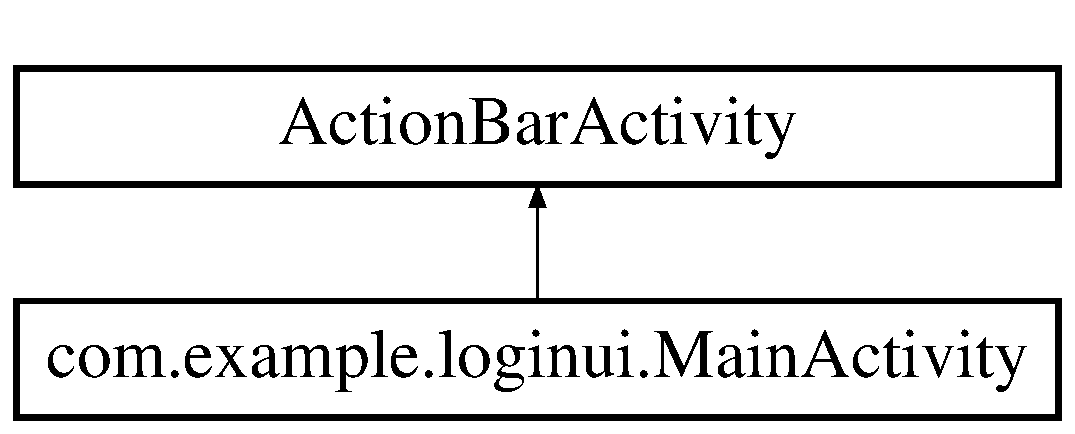
\includegraphics[height=2.000000cm]{classcom_1_1example_1_1loginui_1_1_main_activity}
\end{center}
\end{figure}
\subsection*{Public Member Functions}
\begin{DoxyCompactItemize}
\item 
\hypertarget{classcom_1_1example_1_1loginui_1_1_main_activity_a02ed137deadc6ab361e90e204a756289}{boolean {\bfseries on\+Create\+Options\+Menu} (Menu menu)}\label{classcom_1_1example_1_1loginui_1_1_main_activity_a02ed137deadc6ab361e90e204a756289}

\item 
\hypertarget{classcom_1_1example_1_1loginui_1_1_main_activity_af835cd50ce1bb4bd929a212858f127af}{boolean {\bfseries on\+Options\+Item\+Selected} (Menu\+Item item)}\label{classcom_1_1example_1_1loginui_1_1_main_activity_af835cd50ce1bb4bd929a212858f127af}

\end{DoxyCompactItemize}
\subsection*{Protected Member Functions}
\begin{DoxyCompactItemize}
\item 
\hypertarget{classcom_1_1example_1_1loginui_1_1_main_activity_a1a579a5991445835cfdfa723e874702a}{void {\bfseries on\+Create} (Bundle saved\+Instance\+State)}\label{classcom_1_1example_1_1loginui_1_1_main_activity_a1a579a5991445835cfdfa723e874702a}

\end{DoxyCompactItemize}


The documentation for this class was generated from the following file\+:\begin{DoxyCompactItemize}
\item 
Main\+Activity.\+java\end{DoxyCompactItemize}

\hypertarget{classcom_1_1example_1_1loginui_1_1_password_component}{\section{com.\+example.\+loginui.\+Password\+Component Class Reference}
\label{classcom_1_1example_1_1loginui_1_1_password_component}\index{com.\+example.\+loginui.\+Password\+Component@{com.\+example.\+loginui.\+Password\+Component}}
}
Inheritance diagram for com.\+example.\+loginui.\+Password\+Component\+:\begin{figure}[H]
\begin{center}
\leavevmode
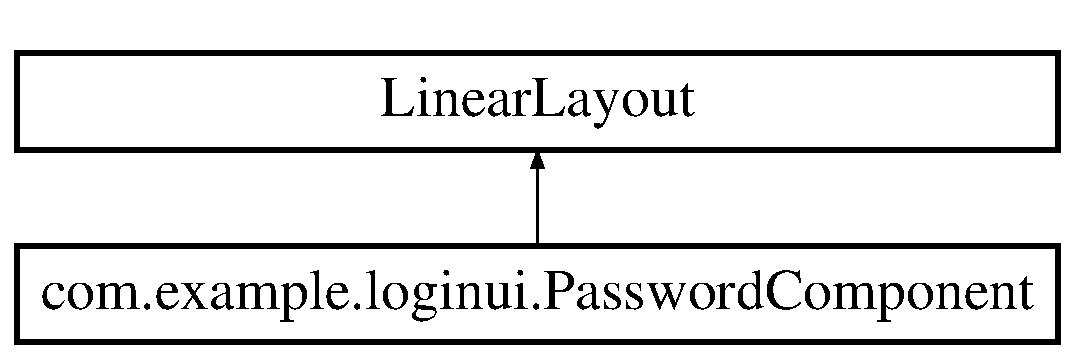
\includegraphics[height=2.000000cm]{classcom_1_1example_1_1loginui_1_1_password_component}
\end{center}
\end{figure}
\subsection*{Public Member Functions}
\begin{DoxyCompactItemize}
\item 
\hyperlink{classcom_1_1example_1_1loginui_1_1_password_component_a592f45b8d066cbe88242f7d4d54e10f6}{Password\+Component} (Context context)
\item 
\hyperlink{classcom_1_1example_1_1loginui_1_1_password_component_aab985a65e134d997d87e9e19dab7109a}{Password\+Component} (Context context, Attribute\+Set attrs)
\item 
void \hyperlink{classcom_1_1example_1_1loginui_1_1_password_component_a9cb40d17af59e93b2a4e9bddc4113d8a}{set\+Text\+Color} (int color)
\item 
Edit\+Text \hyperlink{classcom_1_1example_1_1loginui_1_1_password_component_a7f7fe1e39d271222346e8f28a4d6a350}{get\+Edit\+Text} ()
\item 
Text\+View \hyperlink{classcom_1_1example_1_1loginui_1_1_password_component_aa3b83ce73147bb38a7f99a2db8f5e591}{get\+Check\+Text\+View} ()
\item 
void \hyperlink{classcom_1_1example_1_1loginui_1_1_password_component_a007568a347a47ba2adc2d89f2bb1c499}{set\+Weight} (int edit\+Text\+Weight, int label\+Weight)
\item 
int \hyperlink{classcom_1_1example_1_1loginui_1_1_password_component_af582c35d0504e97d2dc64a576541acf8}{get\+Security\+Color} ()
\item 
int \hyperlink{classcom_1_1example_1_1loginui_1_1_password_component_ae229a011f94d60fc121ff5b90a9f2620}{get\+Security} ()
\item 
String \hyperlink{classcom_1_1example_1_1loginui_1_1_password_component_ae1bd673295ea2d2257da424e082eb4f5}{get\+Security\+Label} ()
\end{DoxyCompactItemize}
\subsection*{Protected Attributes}
\begin{DoxyCompactItemize}
\item 
\hypertarget{classcom_1_1example_1_1loginui_1_1_password_component_ad08e87d64e5d9923aa3a23c58cc8c5bc}{String {\bfseries label\+Not\+Ok}}\label{classcom_1_1example_1_1loginui_1_1_password_component_ad08e87d64e5d9923aa3a23c58cc8c5bc}

\end{DoxyCompactItemize}


\subsection{Constructor \& Destructor Documentation}
\hypertarget{classcom_1_1example_1_1loginui_1_1_password_component_a592f45b8d066cbe88242f7d4d54e10f6}{\index{com\+::example\+::loginui\+::\+Password\+Component@{com\+::example\+::loginui\+::\+Password\+Component}!Password\+Component@{Password\+Component}}
\index{Password\+Component@{Password\+Component}!com\+::example\+::loginui\+::\+Password\+Component@{com\+::example\+::loginui\+::\+Password\+Component}}
\subsubsection[{Password\+Component}]{\setlength{\rightskip}{0pt plus 5cm}com.\+example.\+loginui.\+Password\+Component.\+Password\+Component (
\begin{DoxyParamCaption}
\item[{Context}]{context}
\end{DoxyParamCaption}
)}}\label{classcom_1_1example_1_1loginui_1_1_password_component_a592f45b8d066cbe88242f7d4d54e10f6}
Constructor 
\begin{DoxyParams}{Parameters}
{\em context} & -\/ defines the context \\
\hline
\end{DoxyParams}
\hypertarget{classcom_1_1example_1_1loginui_1_1_password_component_aab985a65e134d997d87e9e19dab7109a}{\index{com\+::example\+::loginui\+::\+Password\+Component@{com\+::example\+::loginui\+::\+Password\+Component}!Password\+Component@{Password\+Component}}
\index{Password\+Component@{Password\+Component}!com\+::example\+::loginui\+::\+Password\+Component@{com\+::example\+::loginui\+::\+Password\+Component}}
\subsubsection[{Password\+Component}]{\setlength{\rightskip}{0pt plus 5cm}com.\+example.\+loginui.\+Password\+Component.\+Password\+Component (
\begin{DoxyParamCaption}
\item[{Context}]{context, }
\item[{Attribute\+Set}]{attrs}
\end{DoxyParamCaption}
)}}\label{classcom_1_1example_1_1loginui_1_1_password_component_aab985a65e134d997d87e9e19dab7109a}
Constructor 
\begin{DoxyParams}{Parameters}
{\em context} & -\/ defines the context \\
\hline
{\em attrs} & -\/ defines the attributes for the component \\
\hline
\end{DoxyParams}


\subsection{Member Function Documentation}
\hypertarget{classcom_1_1example_1_1loginui_1_1_password_component_aa3b83ce73147bb38a7f99a2db8f5e591}{\index{com\+::example\+::loginui\+::\+Password\+Component@{com\+::example\+::loginui\+::\+Password\+Component}!get\+Check\+Text\+View@{get\+Check\+Text\+View}}
\index{get\+Check\+Text\+View@{get\+Check\+Text\+View}!com\+::example\+::loginui\+::\+Password\+Component@{com\+::example\+::loginui\+::\+Password\+Component}}
\subsubsection[{get\+Check\+Text\+View}]{\setlength{\rightskip}{0pt plus 5cm}Text\+View com.\+example.\+loginui.\+Password\+Component.\+get\+Check\+Text\+View (
\begin{DoxyParamCaption}
{}
\end{DoxyParamCaption}
)}}\label{classcom_1_1example_1_1loginui_1_1_password_component_aa3b83ce73147bb38a7f99a2db8f5e591}
Get the right label Text\+View \begin{DoxyReturn}{Returns}
\hyperlink{}{Text\+View} 
\end{DoxyReturn}
\hypertarget{classcom_1_1example_1_1loginui_1_1_password_component_a7f7fe1e39d271222346e8f28a4d6a350}{\index{com\+::example\+::loginui\+::\+Password\+Component@{com\+::example\+::loginui\+::\+Password\+Component}!get\+Edit\+Text@{get\+Edit\+Text}}
\index{get\+Edit\+Text@{get\+Edit\+Text}!com\+::example\+::loginui\+::\+Password\+Component@{com\+::example\+::loginui\+::\+Password\+Component}}
\subsubsection[{get\+Edit\+Text}]{\setlength{\rightskip}{0pt plus 5cm}Edit\+Text com.\+example.\+loginui.\+Password\+Component.\+get\+Edit\+Text (
\begin{DoxyParamCaption}
{}
\end{DoxyParamCaption}
)}}\label{classcom_1_1example_1_1loginui_1_1_password_component_a7f7fe1e39d271222346e8f28a4d6a350}
Get the Edit\+Text of the component \begin{DoxyReturn}{Returns}
\hyperlink{}{Edit\+Text} 
\end{DoxyReturn}
\hypertarget{classcom_1_1example_1_1loginui_1_1_password_component_ae229a011f94d60fc121ff5b90a9f2620}{\index{com\+::example\+::loginui\+::\+Password\+Component@{com\+::example\+::loginui\+::\+Password\+Component}!get\+Security@{get\+Security}}
\index{get\+Security@{get\+Security}!com\+::example\+::loginui\+::\+Password\+Component@{com\+::example\+::loginui\+::\+Password\+Component}}
\subsubsection[{get\+Security}]{\setlength{\rightskip}{0pt plus 5cm}int com.\+example.\+loginui.\+Password\+Component.\+get\+Security (
\begin{DoxyParamCaption}
{}
\end{DoxyParamCaption}
)}}\label{classcom_1_1example_1_1loginui_1_1_password_component_ae229a011f94d60fc121ff5b90a9f2620}
Get value corresponding the Password component's security from 0 to 6 \begin{DoxyReturn}{Returns}
\hyperlink{}{integer} 
\end{DoxyReturn}
\hypertarget{classcom_1_1example_1_1loginui_1_1_password_component_af582c35d0504e97d2dc64a576541acf8}{\index{com\+::example\+::loginui\+::\+Password\+Component@{com\+::example\+::loginui\+::\+Password\+Component}!get\+Security\+Color@{get\+Security\+Color}}
\index{get\+Security\+Color@{get\+Security\+Color}!com\+::example\+::loginui\+::\+Password\+Component@{com\+::example\+::loginui\+::\+Password\+Component}}
\subsubsection[{get\+Security\+Color}]{\setlength{\rightskip}{0pt plus 5cm}int com.\+example.\+loginui.\+Password\+Component.\+get\+Security\+Color (
\begin{DoxyParamCaption}
{}
\end{DoxyParamCaption}
)}}\label{classcom_1_1example_1_1loginui_1_1_password_component_af582c35d0504e97d2dc64a576541acf8}
Get the color corresponding to the Password component security \begin{DoxyReturn}{Returns}
Color \hyperlink{}{integer} 
\end{DoxyReturn}
\hypertarget{classcom_1_1example_1_1loginui_1_1_password_component_ae1bd673295ea2d2257da424e082eb4f5}{\index{com\+::example\+::loginui\+::\+Password\+Component@{com\+::example\+::loginui\+::\+Password\+Component}!get\+Security\+Label@{get\+Security\+Label}}
\index{get\+Security\+Label@{get\+Security\+Label}!com\+::example\+::loginui\+::\+Password\+Component@{com\+::example\+::loginui\+::\+Password\+Component}}
\subsubsection[{get\+Security\+Label}]{\setlength{\rightskip}{0pt plus 5cm}String com.\+example.\+loginui.\+Password\+Component.\+get\+Security\+Label (
\begin{DoxyParamCaption}
{}
\end{DoxyParamCaption}
)}}\label{classcom_1_1example_1_1loginui_1_1_password_component_ae1bd673295ea2d2257da424e082eb4f5}
Get the Password component's security label \begin{DoxyReturn}{Returns}
\hyperlink{}{String} 
\end{DoxyReturn}
\hypertarget{classcom_1_1example_1_1loginui_1_1_password_component_a9cb40d17af59e93b2a4e9bddc4113d8a}{\index{com\+::example\+::loginui\+::\+Password\+Component@{com\+::example\+::loginui\+::\+Password\+Component}!set\+Text\+Color@{set\+Text\+Color}}
\index{set\+Text\+Color@{set\+Text\+Color}!com\+::example\+::loginui\+::\+Password\+Component@{com\+::example\+::loginui\+::\+Password\+Component}}
\subsubsection[{set\+Text\+Color}]{\setlength{\rightskip}{0pt plus 5cm}void com.\+example.\+loginui.\+Password\+Component.\+set\+Text\+Color (
\begin{DoxyParamCaption}
\item[{int}]{color}
\end{DoxyParamCaption}
)}}\label{classcom_1_1example_1_1loginui_1_1_password_component_a9cb40d17af59e93b2a4e9bddc4113d8a}
Set the text color of the component to parameter 
\begin{DoxyParams}{Parameters}
{\em color} & -\/ defines the color of the text \\
\hline
\end{DoxyParams}
\hypertarget{classcom_1_1example_1_1loginui_1_1_password_component_a007568a347a47ba2adc2d89f2bb1c499}{\index{com\+::example\+::loginui\+::\+Password\+Component@{com\+::example\+::loginui\+::\+Password\+Component}!set\+Weight@{set\+Weight}}
\index{set\+Weight@{set\+Weight}!com\+::example\+::loginui\+::\+Password\+Component@{com\+::example\+::loginui\+::\+Password\+Component}}
\subsubsection[{set\+Weight}]{\setlength{\rightskip}{0pt plus 5cm}void com.\+example.\+loginui.\+Password\+Component.\+set\+Weight (
\begin{DoxyParamCaption}
\item[{int}]{edit\+Text\+Weight, }
\item[{int}]{label\+Weight}
\end{DoxyParamCaption}
)}}\label{classcom_1_1example_1_1loginui_1_1_password_component_a007568a347a47ba2adc2d89f2bb1c499}
Sets the weights in the component 
\begin{DoxyParams}{Parameters}
{\em edit\+Text\+Weight} & -\/ defines weight of the \hyperlink{}{Edit\+Text} (right) \\
\hline
{\em label\+Weight} & -\/ -\/ defines weight of the \hyperlink{}{Text\+View} (left) \\
\hline
\end{DoxyParams}


The documentation for this class was generated from the following file\+:\begin{DoxyCompactItemize}
\item 
Password\+Component.\+java\end{DoxyCompactItemize}

\hypertarget{classcom_1_1example_1_1loginui_1_1_registration_component}{\section{com.\+example.\+loginui.\+Registration\+Component Class Reference}
\label{classcom_1_1example_1_1loginui_1_1_registration_component}\index{com.\+example.\+loginui.\+Registration\+Component@{com.\+example.\+loginui.\+Registration\+Component}}
}
Inheritance diagram for com.\+example.\+loginui.\+Registration\+Component\+:\begin{figure}[H]
\begin{center}
\leavevmode
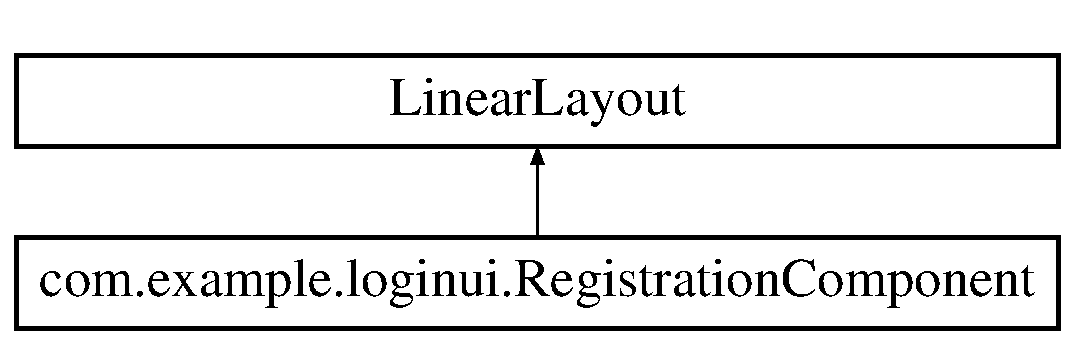
\includegraphics[height=2.000000cm]{classcom_1_1example_1_1loginui_1_1_registration_component}
\end{center}
\end{figure}
\subsection*{Public Member Functions}
\begin{DoxyCompactItemize}
\item 
\hyperlink{classcom_1_1example_1_1loginui_1_1_registration_component_a41281e46f8f4f3ab43362a73150b33dd}{Registration\+Component} (Context context)
\item 
\hyperlink{classcom_1_1example_1_1loginui_1_1_registration_component_ac8b35f033ff3377bc24452941a2755fd}{Registration\+Component} (Context context, Attribute\+Set attrs)
\item 
void \hyperlink{classcom_1_1example_1_1loginui_1_1_registration_component_a2cf46eb87d908d2a41116ae768aa4a7c}{set\+Header\+Color} (int color)
\item 
void \hyperlink{classcom_1_1example_1_1loginui_1_1_registration_component_a59f6917d7327378eacbf8694ee407687}{set\+Text\+Color} (int color)
\item 
void \hyperlink{classcom_1_1example_1_1loginui_1_1_registration_component_af7bb62c95c652c4928c4038ce8343e5d}{set\+Field\+Background\+Color} (int color)
\item 
void \hyperlink{classcom_1_1example_1_1loginui_1_1_registration_component_a0eef8c76a87323d299a10b3f8828986b}{on\+Create} (Context context)
\item 
void \hyperlink{classcom_1_1example_1_1loginui_1_1_registration_component_a51cfbb68ec30e0266047661aee3e26b3}{add\+Field} (String fieldname)
\item 
void \hyperlink{classcom_1_1example_1_1loginui_1_1_registration_component_a03275021d51f8085a7a706730ac41f81}{add\+Field} (String fieldname, Boolean required)
\end{DoxyCompactItemize}


\subsection{Constructor \& Destructor Documentation}
\hypertarget{classcom_1_1example_1_1loginui_1_1_registration_component_a41281e46f8f4f3ab43362a73150b33dd}{\index{com\+::example\+::loginui\+::\+Registration\+Component@{com\+::example\+::loginui\+::\+Registration\+Component}!Registration\+Component@{Registration\+Component}}
\index{Registration\+Component@{Registration\+Component}!com\+::example\+::loginui\+::\+Registration\+Component@{com\+::example\+::loginui\+::\+Registration\+Component}}
\subsubsection[{Registration\+Component}]{\setlength{\rightskip}{0pt plus 5cm}com.\+example.\+loginui.\+Registration\+Component.\+Registration\+Component (
\begin{DoxyParamCaption}
\item[{Context}]{context}
\end{DoxyParamCaption}
)}}\label{classcom_1_1example_1_1loginui_1_1_registration_component_a41281e46f8f4f3ab43362a73150b33dd}
Constructor of Registration component 
\begin{DoxyParams}{Parameters}
{\em context} & \\
\hline
\end{DoxyParams}
\hypertarget{classcom_1_1example_1_1loginui_1_1_registration_component_ac8b35f033ff3377bc24452941a2755fd}{\index{com\+::example\+::loginui\+::\+Registration\+Component@{com\+::example\+::loginui\+::\+Registration\+Component}!Registration\+Component@{Registration\+Component}}
\index{Registration\+Component@{Registration\+Component}!com\+::example\+::loginui\+::\+Registration\+Component@{com\+::example\+::loginui\+::\+Registration\+Component}}
\subsubsection[{Registration\+Component}]{\setlength{\rightskip}{0pt plus 5cm}com.\+example.\+loginui.\+Registration\+Component.\+Registration\+Component (
\begin{DoxyParamCaption}
\item[{Context}]{context, }
\item[{Attribute\+Set}]{attrs}
\end{DoxyParamCaption}
)}}\label{classcom_1_1example_1_1loginui_1_1_registration_component_ac8b35f033ff3377bc24452941a2755fd}
Constructor of Registration component


\begin{DoxyParams}{Parameters}
{\em context} & \hyperlink{}{Context} \\
\hline
{\em attrs} & \hyperlink{}{attr} \\
\hline
\end{DoxyParams}


\subsection{Member Function Documentation}
\hypertarget{classcom_1_1example_1_1loginui_1_1_registration_component_a51cfbb68ec30e0266047661aee3e26b3}{\index{com\+::example\+::loginui\+::\+Registration\+Component@{com\+::example\+::loginui\+::\+Registration\+Component}!add\+Field@{add\+Field}}
\index{add\+Field@{add\+Field}!com\+::example\+::loginui\+::\+Registration\+Component@{com\+::example\+::loginui\+::\+Registration\+Component}}
\subsubsection[{add\+Field}]{\setlength{\rightskip}{0pt plus 5cm}void com.\+example.\+loginui.\+Registration\+Component.\+add\+Field (
\begin{DoxyParamCaption}
\item[{String}]{fieldname}
\end{DoxyParamCaption}
)}}\label{classcom_1_1example_1_1loginui_1_1_registration_component_a51cfbb68ec30e0266047661aee3e26b3}
Function to add a new field


\begin{DoxyParams}{Parameters}
{\em fieldname} & -\/ sets the name of the field \hyperlink{}{string} \\
\hline
\end{DoxyParams}
\hypertarget{classcom_1_1example_1_1loginui_1_1_registration_component_a03275021d51f8085a7a706730ac41f81}{\index{com\+::example\+::loginui\+::\+Registration\+Component@{com\+::example\+::loginui\+::\+Registration\+Component}!add\+Field@{add\+Field}}
\index{add\+Field@{add\+Field}!com\+::example\+::loginui\+::\+Registration\+Component@{com\+::example\+::loginui\+::\+Registration\+Component}}
\subsubsection[{add\+Field}]{\setlength{\rightskip}{0pt plus 5cm}void com.\+example.\+loginui.\+Registration\+Component.\+add\+Field (
\begin{DoxyParamCaption}
\item[{String}]{fieldname, }
\item[{Boolean}]{required}
\end{DoxyParamCaption}
)}}\label{classcom_1_1example_1_1loginui_1_1_registration_component_a03275021d51f8085a7a706730ac41f81}
Function to add a new field


\begin{DoxyParams}{Parameters}
{\em fieldname} & -\/ sets the name of the field \hyperlink{}{string} \\
\hline
{\em required} & -\/ true makes it a required field \hyperlink{}{bool} \\
\hline
\end{DoxyParams}
\hypertarget{classcom_1_1example_1_1loginui_1_1_registration_component_a0eef8c76a87323d299a10b3f8828986b}{\index{com\+::example\+::loginui\+::\+Registration\+Component@{com\+::example\+::loginui\+::\+Registration\+Component}!on\+Create@{on\+Create}}
\index{on\+Create@{on\+Create}!com\+::example\+::loginui\+::\+Registration\+Component@{com\+::example\+::loginui\+::\+Registration\+Component}}
\subsubsection[{on\+Create}]{\setlength{\rightskip}{0pt plus 5cm}void com.\+example.\+loginui.\+Registration\+Component.\+on\+Create (
\begin{DoxyParamCaption}
\item[{Context}]{context}
\end{DoxyParamCaption}
)}}\label{classcom_1_1example_1_1loginui_1_1_registration_component_a0eef8c76a87323d299a10b3f8828986b}
Creates the standard registration fields


\begin{DoxyParams}{Parameters}
{\em context} & -\/ context \hyperlink{}{Context} \\
\hline
\end{DoxyParams}
\hypertarget{classcom_1_1example_1_1loginui_1_1_registration_component_af7bb62c95c652c4928c4038ce8343e5d}{\index{com\+::example\+::loginui\+::\+Registration\+Component@{com\+::example\+::loginui\+::\+Registration\+Component}!set\+Field\+Background\+Color@{set\+Field\+Background\+Color}}
\index{set\+Field\+Background\+Color@{set\+Field\+Background\+Color}!com\+::example\+::loginui\+::\+Registration\+Component@{com\+::example\+::loginui\+::\+Registration\+Component}}
\subsubsection[{set\+Field\+Background\+Color}]{\setlength{\rightskip}{0pt plus 5cm}void com.\+example.\+loginui.\+Registration\+Component.\+set\+Field\+Background\+Color (
\begin{DoxyParamCaption}
\item[{int}]{color}
\end{DoxyParamCaption}
)}}\label{classcom_1_1example_1_1loginui_1_1_registration_component_af7bb62c95c652c4928c4038ce8343e5d}
Function to set background color for each field


\begin{DoxyParams}{Parameters}
{\em color} & -\/ defines the color \hyperlink{}{integer} \\
\hline
\end{DoxyParams}
\hypertarget{classcom_1_1example_1_1loginui_1_1_registration_component_a2cf46eb87d908d2a41116ae768aa4a7c}{\index{com\+::example\+::loginui\+::\+Registration\+Component@{com\+::example\+::loginui\+::\+Registration\+Component}!set\+Header\+Color@{set\+Header\+Color}}
\index{set\+Header\+Color@{set\+Header\+Color}!com\+::example\+::loginui\+::\+Registration\+Component@{com\+::example\+::loginui\+::\+Registration\+Component}}
\subsubsection[{set\+Header\+Color}]{\setlength{\rightskip}{0pt plus 5cm}void com.\+example.\+loginui.\+Registration\+Component.\+set\+Header\+Color (
\begin{DoxyParamCaption}
\item[{int}]{color}
\end{DoxyParamCaption}
)}}\label{classcom_1_1example_1_1loginui_1_1_registration_component_a2cf46eb87d908d2a41116ae768aa4a7c}
Function to set text color of the headers 
\begin{DoxyParams}{Parameters}
{\em color} & -\/ defines the color \hyperlink{}{integer} \\
\hline
\end{DoxyParams}
\hypertarget{classcom_1_1example_1_1loginui_1_1_registration_component_a59f6917d7327378eacbf8694ee407687}{\index{com\+::example\+::loginui\+::\+Registration\+Component@{com\+::example\+::loginui\+::\+Registration\+Component}!set\+Text\+Color@{set\+Text\+Color}}
\index{set\+Text\+Color@{set\+Text\+Color}!com\+::example\+::loginui\+::\+Registration\+Component@{com\+::example\+::loginui\+::\+Registration\+Component}}
\subsubsection[{set\+Text\+Color}]{\setlength{\rightskip}{0pt plus 5cm}void com.\+example.\+loginui.\+Registration\+Component.\+set\+Text\+Color (
\begin{DoxyParamCaption}
\item[{int}]{color}
\end{DoxyParamCaption}
)}}\label{classcom_1_1example_1_1loginui_1_1_registration_component_a59f6917d7327378eacbf8694ee407687}
Function to set text color


\begin{DoxyParams}{Parameters}
{\em color} & -\/ defines the color \hyperlink{}{integer} \\
\hline
\end{DoxyParams}


The documentation for this class was generated from the following file\+:\begin{DoxyCompactItemize}
\item 
Registration\+Component.\+java\end{DoxyCompactItemize}

%--- End generated contents ---

% Index
\newpage
\phantomsection
\addcontentsline{toc}{chapter}{Index}
\printindex

\end{document}
